% Biên dịch bằng XeLaTeX (Overleaf: Menu > Compiler > XeLaTeX; tệp latexmkrc đã đặt sẵn).
% Các chỗ chữ đỏ [..] cần điền: link repo, URL production, ngày Sprint, link minh chứng, video.
\documentclass[a4paper]{article}
\usepackage{iftex}
\ifPDFTeX
  \usepackage{vntex}% pdfLaTeX: gói tiếng Việt của template
\else
  \usepackage{fontspec}% XeLaTeX/LuaLaTeX: dùng Latin Modern (có đủ dấu tiếng Việt)
  \setmainfont{Latin Modern Roman}\setsansfont{Latin Modern Sans}\setmonofont{Latin Modern Mono}
\fi
\usepackage{a4wide,amssymb,epsfig,latexsym,multicol,array,hhline,fancyhdr}
\usepackage{booktabs}
\usepackage{amsmath}
\usepackage{lastpage}
\usepackage{enumerate}
\usepackage{color}
\usepackage{graphicx}
\usepackage{array}
\usepackage{tabularx, caption}
\usepackage{subcaption}
\usepackage{longtable}
\usepackage{multirow}
\usepackage[framemethod=tikz]{mdframed}
\usepackage{rotating}
\usepackage{geometry}
\geometry{a4paper,left=2.2cm,right=2.2cm,top=2.6cm,bottom=2.4cm,headheight=40pt}
\usepackage{setspace}
\usepackage{tikz}
\usepackage{listings}
\usetikzlibrary{arrows.meta,positioning,shapes.geometric,calc,backgrounds}
\usepackage{hyperref}
\hypersetup{urlcolor=blue,linkcolor=black,citecolor=black,colorlinks=true}

\newtheorem{theorem}{{\bf Định lý}}
\newtheorem{property}{{\bf Tính chất}}
\newtheorem{proposition}{{\bf Mệnh đề}}
\newtheorem{corollary}[proposition]{{\bf Hệ quả}}
\newtheorem{lemma}[proposition]{{\bf Bổ đề}}

%%% ====== THÔNG TIN NHÓM: sửa các dòng màu đỏ [..] trước khi nộp ======
\newcommand{\TODO}[1]{\textcolor{red}{[#1]}}
\newcommand{\GVHD}{Từ Lãng Phiêu}
\newcommand{\st}[1]{\texttt{#1}}
\newcommand{\ra}{\ensuremath{\rightarrow}}

\setlength{\headheight}{40pt}
\pagestyle{fancy}
\fancyhead{}
\fancyhead[L]{
 \begin{tabular}{rl}
    \begin{picture}(25,15)(0,0)
    \put(0,-8){
\includegraphics[width=8mm, height=8mm]{logoITSGUsmall.png}}
   \end{picture}&
	\begin{tabular}{l}
		\textbf{\bf \ttfamily Trường Đại học Sài Gòn}\\
		\textbf{\bf \ttfamily Khoa Công Nghệ Thông Tin}
	\end{tabular}
 \end{tabular}
}
\fancyhead[R]{\begin{tabular}{l}\tiny \bf \\ \tiny \bf \end{tabular}}
\fancyfoot{}
\fancyfoot[L]{\scriptsize \ttfamily Bài tập lớn môn Công nghệ Phần mềm - Học kỳ I, năm học 2026-2027}
\fancyfoot[R]{\scriptsize \ttfamily Trang {\thepage}/\pageref{LastPage}}
\renewcommand{\headrulewidth}{0.3pt}
\renewcommand{\footrulewidth}{0.3pt}

\setcounter{secnumdepth}{4}
\setcounter{tocdepth}{2}
\renewcommand{\contentsname}{Mục lục}
\renewcommand{\refname}{Tài liệu tham khảo}
\renewcommand{\figurename}{Hình}
\renewcommand{\tablename}{Bảng}
\renewcommand{\lstlistingname}{Mã nguồn}

\definecolor{dkgreen}{rgb}{0,0.6,0}
\definecolor{gray}{rgb}{0.5,0.5,0.5}
\definecolor{mauve}{rgb}{0.58,0,0.82}
\definecolor{brew}{rgb}{0.435,0.271,0.153}
\definecolor{okgreen}{rgb}{0.1,0.55,0.3}
\definecolor{warnred}{rgb}{0.75,0.15,0.15}

\lstset{frame=tb, language={}, aboveskip=3mm, belowskip=3mm, showstringspaces=false, columns=flexible,
  basicstyle={\footnotesize\ttfamily}, numbers=left, numberstyle=\tiny\color{gray}, keywordstyle=\color{blue},
  commentstyle=\color{dkgreen}, stringstyle=\color{mauve}, breaklines=true, breakatwhitespace=true, tabsize=2,
  numbersep=5pt, xleftmargin=1.5em}

\renewcommand{\arraystretch}{1.25}
\newcolumntype{L}[1]{>{\raggedright\arraybackslash}p{#1}}
\newcommand{\hl}[1]{\rowcolor{brew!12}#1}
\usepackage{colortbl}
\usepackage{float}
\usepackage{fancyvrb}
\usepackage{xurl}


% --- Macro chèn sơ đồ ---
\newcommand{\dfig}[4][1]{\begin{figure}[H]\centering\includegraphics[width=#1\textwidth,height=0.82\textheight,keepaspectratio]{diagrams/#2}\caption{#3}\label{#4}\end{figure}}
\newcommand{\shot}[2]{\fbox{\includegraphics[width=#2]{shots/#1}}}
\newcommand{\evidenceimg}[2]{\IfFileExists{shots/#1}{\begin{center}\fbox{\includegraphics[width=0.9\textwidth,height=0.42\textheight,keepaspectratio]{shots/#1}}\\[3pt]{\small #2}\end{center}}{\evidence{#2\\(ảnh: \texttt{shots/#1})}}}
\newcommand{\evidence}[1]{\begin{center}\fcolorbox{warnred}{warnred!6}{\parbox{0.92\textwidth}{\centering\vspace{1.2cm}\textcolor{warnred}{\textbf{[Chèn ảnh minh chứng]}}\\[2pt]\small #1\vspace{1.2cm}}}\end{center}}
\newcommand{\sfig}[3]{\begin{sidewaysfigure}\centering\includegraphics[width=0.96\textheight,height=0.78\textwidth,keepaspectratio]{diagrams/#1}\caption{#2}\label{#3}\end{sidewaysfigure}}
\begin{document}
\sloppy\setlength{\emergencystretch}{3em}\setlength{\fboxsep}{0pt}

%%%%%%%%%%%%%%%%%%%% TRANG BÌA %%%%%%%%%%%%%%%%%%%%
\begin{titlepage}
\begin{center}
TRƯỜNG ĐẠI HỌC SÀI GÒN \\
KHOA CÔNG NGHỆ THÔNG TIN
\end{center}
\vspace{1cm}
\begin{figure}[h!]
\begin{center}

\includegraphics[width=3cm]{logoITSGU.png}
\end{center}
\end{figure}
\vspace{1cm}
\begin{center}
\begin{tabular}{c}
	\textbf{{\Large CÔNG NGHỆ PHẦN MỀM}}\\
	~~\\
	\hline
	\\
	\textbf{{\Large Bài tập lớn: BrewLite -- Assignment 2}}\\
	\\
	\textbf{{\Huge Requirements to Deployment}}\\
	\\
	\textbf{{\Large Từ yêu cầu đến triển khai -- phiên bản 2.0}}\\
	\\
	\hline
\end{tabular}
\end{center}
\vspace{2.5cm}
\begin{table}[h]
\begin{tabular}{rrl}
\hspace{5 cm} & GVHD: & \GVHD \\
& SV: & Lâm Sơn Hùng - 3123560031 \\
\end{tabular}
\vspace{1.5 cm}
\end{table}
\begin{center}
{\footnotesize TP. HỒ CHÍ MINH, THÁNG 11/2026}
\end{center}
\end{titlepage}

\thispagestyle{empty}
\newpage
\tableofcontents
\newpage

%%%%%%%%%%%%%%%%%%%% 1. TỔNG QUAN %%%%%%%%%%%%%%%%%%%%
\section{Tổng quan Assignment 2}

\subsection{Mục tiêu}
Assignment 2 tiếp tục đề tài BrewLite của Assignment 1 và đi hết một chuỗi công việc hoàn chỉnh: khai thác yêu cầu, mô hình hóa, thiết kế kiến trúc, hiện thực qua hai Sprint, thiết lập CI/CD và triển khai lên môi trường production truy cập được qua HTTPS. Luồng nghiệp vụ tối thiểu:
\begin{center}
\textbf{Xem menu \ra{} Chọn tùy chọn \ra{} Giỏ hàng \ra{} Đặt đơn \ra{} Thanh toán \ra{} Theo dõi đơn}
\end{center}
Ba thành phần bắt buộc được giữ nguyên: Next.js (mobile-first/PWA), NestJS và PostgreSQL. Công nghệ bổ sung: Docker, GitHub Actions, GitHub Container Registry (GHCR), Render, Playwright, Vitest, PlantUML.

\subsection{Thông tin bàn giao}
\begin{center}
\begin{tabular}{|L{4.2cm}|L{10.8cm}|}
\hline
Repository & \url{https://github.com/kaiqwwp/brewlite} \\ \hline
Web production (HTTPS) & \url{https://brewlite-web-ed96.onrender.com} \\ \hline
API production & \url{https://brewlite-api-9uli.onrender.com} -- health check: \st{/health} \\ \hline
Phiên bản & \st{v2.0.0} (release notes: \st{docs/releases/v2.0.0.md}) \\ \hline
Video demo & \url{https://github.com/kaiqwwp/brewlite/blob/main/docs/evidence/video.md} \\ \hline
Tài khoản nhân viên mẫu & \st{staff@brewlite.local} / mật khẩu đặt trong biến \st{STAFF\_PASSWORD} trên Render \\ \hline
\end{tabular}
\end{center}

\subsection{Quy trình năm task}
Năm task thực hiện tuần tự; mỗi task kết thúc bằng một commit (hoặc pull request) đưa tạo phẩm vào repository, nên lịch sử git phản ánh đúng thứ tự (Bảng~\ref{tab:history}).

\begin{table}[H]
\centering
\begin{tabular}{|c|L{3.3cm}|L{6.3cm}|L{3.8cm}|}
\hline
\textbf{Task} & \textbf{Giai đoạn} & \textbf{Tạo phẩm chính} & \textbf{Vị trí trong repo} \\ \hline
1 & Khai thác và đặc tả yêu cầu & Bối cảnh, stakeholder, phạm vi, SRS (FR/NFR, MoSCoW), use-case tổng quát, đặc tả UC-05 & \st{docs/requirements/} \\ \hline
2 & Mô hình hóa hệ thống & Activity, sequence, class diagram (PlantUML + SVG) & \st{docs/diagrams/} \\ \hline
3 & Thiết kế kiến trúc & Kiến trúc C4 + phân lớp, 7 ADR, deployment diagram & \st{docs/architecture/} \\ \hline
4 & Sprint 1 & Repo, quy ước, CI, MVP xem menu, test & \st{apps/}, \st{ci.yml} \\ \hline
5 & Sprint 2 và Delivery & MVP hoàn chỉnh, migration, health, PWA, E2E, CD, production, bàn giao & \st{apps/}, \st{tests/e2e/}, \st{cd.yml}, \st{render.yaml} \\ \hline
\end{tabular}
\caption{Năm task và tạo phẩm}
\end{table}

\begin{table}[H]
\centering
\small
\begin{tabular}{|l|L{12.6cm}|}
\hline
\textbf{Commit} & \textbf{Nội dung} \\ \hline
\st{39c2c2e} (tag \st{v1.0.0}) & Bản nộp Assignment 1 \\ \hline
\st{11ced65} & chore: chuyển repo sang cấu trúc \st{apps/web}, \st{apps/api}, \st{docs} \\ \hline
\st{cab59f0} & docs(task1): bối cảnh, stakeholder, phạm vi, SRS và đặc tả UC-05 \\ \hline
\st{f826db1} & docs(task2): activity, sequence và class diagram \\ \hline
\st{690090b} & docs(task3): kiến trúc C4 + phân lớp, 7 ADR, deployment diagram production \\ \hline
\st{413c13e} & chore(task4): quy ước repo, CI cho pull request, lint và test frontend (Sprint 1) \\ \hline
\st{6dcbca4} & feat(task5): migration, LoyaltyTransaction, health, PWA, E2E và pipeline CD (Sprint 2) \\ \hline
\end{tabular}
\caption{Lịch sử commit theo thứ tự task (\st{git log --oneline})}
\label{tab:history}
\end{table}

\subsection{Kế thừa từ Assignment 1}
Các chức năng menu, chi tiết, giỏ hàng, xác thực JWT, tạo đơn, thanh toán idempotent, state machine đơn hàng, tồn kho đồng thời, khuyến mãi và điểm thưởng được giữ nguyên từ Assignment 1 (34 test tự động, 55 kịch bản kiểm thử giao diện, 6 lỗi nghiệp vụ đã sửa). Assignment 2 thay đổi hoặc bổ sung:
\begin{itemize}
  \item Cấu trúc repo \st{frontend/}, \st{backend/} \ra{} \st{apps/web}, \st{apps/api}; thêm \st{docs/}, \st{tests/e2e}, \st{.github/workflows}.
  \item CSDL: bỏ \st{synchronize}, quản lý schema bằng migration; thêm khóa ngoại và ràng buộc CHECK; bảng \st{coupons} đổi tên thành \st{promotions}; bảng mới \st{loyalty\_transactions}.
  \item Health check có kiểm tra CSDL, log JSON, kiểm tra cấu hình khi khởi động, PWA.
  \item ESLint, test component frontend, E2E Playwright, CI/CD và triển khai production.
\end{itemize}

%%%%%%%%%%%%%%%%%%%% 2. TASK 1 %%%%%%%%%%%%%%%%%%%%
\section{Task 1 -- Khai thác và đặc tả yêu cầu}

\subsection{Task 1.1 -- Bối cảnh, stakeholder và phạm vi}
\textbf{Vấn đề nghiệp vụ.} Quán cà phê nhỏ vào giờ cao điểm (7h--9h, 11h30--13h) có hàng dài trước quầy; mỗi khách mất 1--3 phút để gọi món và trả tiền. Khách bỏ về khi thấy hàng dài, nhân viên vừa nhận order vừa thu tiền nên dễ nhầm món, size, topping, và quán không có dữ liệu đơn hàng hay chương trình khách hàng thân thiết. BrewLite cho khách đặt và thanh toán trước trên điện thoại, chỉ tới quầy nhận đồ uống.

\textbf{Product Vision:} ``BrewLite giúp khách hàng đặt và thanh toán đồ uống không dùng tiền mặt chỉ trong vài chạm, giảm thời gian xếp hàng và nhận đơn nhanh tại quầy.''

\begin{longtable}{|L{2.6cm}|L{3.6cm}|L{6.4cm}|L{1.6cm}|}
\hline
\textbf{Stakeholder} & \textbf{Mục tiêu} & \textbf{Kỳ vọng với hệ thống} & \textbf{Ảnh hưởng} \\ \hline
\endhead
Khách hàng & Mua nhanh, không xếp hàng, không mang tiền mặt & Menu rõ giá; chọn size/topping dễ; thanh toán an toàn, không bị trừ tiền hai lần; biết khi nào đơn sẵn sàng; dùng tốt trên điện thoại & Cao \\ \hline
Nhân viên quầy & Biết đơn nào đã trả tiền, pha đúng món & Danh sách đơn đã thanh toán đúng size/topping; đổi trạng thái \st{PREPARING} \ra{} \st{READY} \ra{} \st{COMPLETED} & Trung bình \\ \hline
Quản lý cửa hàng & Tăng doanh thu giờ cao điểm, giữ khách quay lại & Không bán vượt tồn kho; khuyến mãi và điểm thưởng tính đúng; dữ liệu đơn hàng được lưu & Cao \\ \hline
Giảng viên / khách hàng nghiệm thu & Đánh giá quy trình và sản phẩm & Tạo phẩm đúng thứ tự Task 1\ra5; truy vết được; URL production chạy; CI/CD hoạt động & Cao \\ \hline
Nhóm phát triển (1 người) & Hoàn thành đúng hạn, chất lượng & Yêu cầu rõ, có tiêu chí chấp nhận; pipeline tự động; triển khai lặp lại được & Cao \\ \hline
Đơn vị thanh toán & Xử lý giao dịch & Mỗi giao dịch có mã định danh; yêu cầu lặp không bị tính tiền hai lần (MVP dùng cổng mô phỏng) & Trung bình \\ \hline
\caption{Stakeholder, mục tiêu và kỳ vọng}
\end{longtable}

\textbf{Phạm vi MVP (in-scope):} xem menu (FR-01); chi tiết, size, topping (FR-02); giỏ hàng (FR-03); đăng ký/đăng nhập JWT (FR-04); đặt đơn với giá do server tính, giữ tồn kho, chống tạo đơn trùng (FR-05) và mã giảm giá (FR-06); thanh toán Ví/Thẻ mô phỏng, idempotent (FR-07); xác nhận, trạng thái, lịch sử đơn (FR-08, FR-09); state machine đơn hàng và hủy đơn (FR-10, FR-11); điểm thưởng (FR-12); PWA (FR-13); health check, log, CI/CD, triển khai HTTPS.

\textbf{Phạm vi mở rộng (backlog):} giao diện nhân viên quầy; cổng thanh toán thật và hoàn tiền; thông báo khi đơn \st{READY}; đơn \st{PENDING} tự hết hạn; giỏ hàng theo tài khoản; cookie HttpOnly + refresh token; trang quản trị menu.

\textbf{Không thực hiện (out-of-scope):} giao hàng tận nơi; thanh toán tiền mặt; nhiều chi nhánh; ứng dụng native (thay bằng PWA); quản lý nguyên liệu, kế toán; lưu thông tin thẻ của khách.

\begin{table}[H]
\centering\small
\begin{tabular}{|c|L{13.6cm}|}
\hline
\textbf{Mã} & \textbf{Giả định (A) và ràng buộc (C)} \\ \hline
A-01 & Khách có điện thoại thông minh với trình duyệt hiện đại và có Internet. \\ \hline
A-02 & Một quán, một menu; tồn kho tính theo số ly bán được của từng sản phẩm. \\ \hline
A-03 & Cổng thanh toán mô phỏng hành xử như cổng thật: trả kết quả đồng bộ, mỗi yêu cầu có mã tham chiếu. \\ \hline
A-04 & Nhân viên dùng API để cập nhật trạng thái pha chế trong MVP. \\ \hline
A-05 & Lưu lượng MVP dưới 50 người dùng đồng thời, đủ cho gói miễn phí. \\ \hline
C-01 & Bắt buộc Next.js (mobile-first/PWA), NestJS, PostgreSQL. \\ \hline
C-02 & Agile Scrum, 2 Sprint; 5 task tuần tự, task sau chỉ nghiệm thu khi tạo phẩm task trước có trên repo. \\ \hline
C-03 & Nhóm 1 người; ngân sách hạ tầng 0 đồng (GitHub Actions, GHCR, Render gói miễn phí). \\ \hline
C-04 & Mọi thay đổi yêu cầu, sơ đồ, kiến trúc đi qua commit/pull request có lý do. \\ \hline
C-05 & Secret không nằm trong repository hay log CI. \\ \hline
C-06 & Giao diện tiếng Việt, tiền tệ VND. \\ \hline
\end{tabular}
\caption{Giả định và ràng buộc}
\end{table}

\begin{longtable}{|c|L{5.4cm}|c|c|L{5.6cm}|}
\hline
\textbf{Mã} & \textbf{Rủi ro} & \textbf{KN} & \textbf{AH} & \textbf{Biện pháp} \\ \hline
\endhead
R-01 & Khách bấm thanh toán nhiều lần hoặc mất mạng gây trừ tiền hai lần & Cao & Cao & Idempotency-Key bắt buộc, ràng buộc UNIQUE, khóa dòng đơn \\ \hline
R-02 & Nhiều khách đặt cùng lúc sản phẩm sắp hết gây bán vượt kho & TB & Cao & Optimistic locking (\st{version}), \st{CHECK stock >= 0}, rollback cả đơn \\ \hline
R-03 & Một người làm, khối lượng lớn, dễ trễ hạn & Cao & Cao & Ưu tiên MoSCoW; tự động hóa kiểm thử và triển khai \\ \hline
R-04 & Gói miễn phí Render ngủ sau 15 phút; Postgres miễn phí hết hạn sau 30 ngày & Cao & TB & Smoke test có thử lại; mở URL trước buổi chấm; hướng dẫn tạo lại CSDL \\ \hline
R-05 & Lộ secret khi commit hoặc trong log & Thấp & Cao & \st{.env} trong \st{.gitignore}, gitleaks trong CI, secret chỉ ở GitHub Secrets/Render \\ \hline
R-06 & Migration lỗi làm hỏng CSDL production & Thấp & Cao & Migration chạy trong một transaction; health check chặn bản lỗi; có lệnh revert \\ \hline
R-07 & Giá trên giao diện lệch giá server & TB & TB & Server luôn tính lại giá; giao diện yêu cầu khách xác nhận giá mới \\ \hline
\caption{Rủi ro ban đầu (KN: khả năng, AH: ảnh hưởng, TB: trung bình)}
\end{longtable}

\subsection{Task 1.2 -- Yêu cầu chức năng và phi chức năng (SRS rút gọn)}
Mức ưu tiên theo MoSCoW. Mỗi yêu cầu có tiêu chí chấp nhận kiểm chứng được và mã test tương ứng: \st{UT-xx} unit test API, \st{INT-Txx} integration test API với PostgreSQL, \st{FE-Txx} test component web, \st{E2E-T01} Playwright, \st{UI-<nhóm>} bộ 55 kịch bản giao diện của Assignment 1.

{\small
\begin{longtable}{|L{1.1cm}|L{3.3cm}|L{1.15cm}|L{6.6cm}|L{2.2cm}|}
\hline
\textbf{Mã} & \textbf{Yêu cầu} & \textbf{Ưu tiên} & \textbf{Tiêu chí chấp nhận} & \textbf{Test} \\ \hline
\endhead
FR-01 & Xem menu: ảnh, tên, giá size M, nhãn ``Hết hàng'' & Must & \st{GET /products} trả 200 với \st{\{id, name, price, imageUrl, stock\}}; màn hình có trạng thái đang tải, rỗng, lỗi + ``Thử lại''; 360px hiển thị 2 cột, không cuộn ngang & INT-T01, FE-T01, E2E-T01, UI-A \\ \hline
FR-02 & Chi tiết sản phẩm, chọn size S/M/L và topping & Must & \st{GET /products/:id} trả \st{options.sizes} (S $-$5.000đ, M 0, L +7.000đ) và 4 topping; id sai trả 404; đơn giá = giá gốc + size + tổng topping (mỗi loại một lần); hết hàng thì vô hiệu nút thêm & INT-T01, UT-05..07, UI-A \\ \hline
FR-03 & Giỏ hàng & Must & Gộp cùng món + size + bộ topping; số lượng 1--20, về 0 thì xóa; tổng = $\Sigma$ đơn giá $\times$ số lượng; giữ khi tải lại trang & FE-T02, UI-B \\ \hline
FR-04 & Đăng ký, đăng nhập, JWT & Must & Đăng ký trả 201 + \st{accessToken}; email trùng 409; dữ liệu sai 400; sai mật khẩu 401; mật khẩu băm bcrypt; thiếu/sai token 401; token hết hạn thì tự đăng xuất & INT-T02..04, UI-C \\ \hline
FR-05 & Đặt đơn: giá server, giữ tồn kho & Must & \st{POST /orders} trả 201, đơn \st{PENDING}, tổng do server tính; dữ liệu sai 400/404; thiếu hàng 409 \st{OUT\_OF\_STOCK} không trừ dòng nào; cùng \st{Idempotency-Key} (kể cả 5 yêu cầu đồng thời) chỉ một đơn; tồn kho không âm; chưa đăng nhập thì chuyển \st{/login} rồi quay lại & INT-T05, T06, T14, T15, T18--T20, T25, E2E-T01 \\ \hline
FR-06 & Mã giảm giá & Should & BREW10 10\% tối đa 20.000đ; WELCOME20 20\% cho đơn từ 100.000đ, tối đa 50.000đ; làm tròn xuống; mã sai/hết hạn/chưa đủ tối thiểu trả 400 & UT-08..10, INT-T21, T23 \\ \hline
FR-07 & Thanh toán Ví/Thẻ mô phỏng, idempotent & Must & Bắt buộc \st{Idempotency-Key} (thiếu 400); thành công 201, đơn \st{PAID}; thất bại 402, đơn \st{PAYMENT\_FAILED}; gửi lại cùng key trả kết quả cũ (200 + \st{Idempotent-Replayed}), chỉ một payment; key dùng cho đơn khác 409; thử lại bằng key mới \ra{} \st{PAID} & INT-T08..10, T16, T17 \\ \hline
FR-08 & Xác nhận và trạng thái đơn & Must & Chuyển \st{/orders/:id}, hiện ``Đã thanh toán''; chỉ chủ đơn hoặc nhân viên xem được (403/404) & E2E-T01, UI-E \\ \hline
FR-09 & Lịch sử đơn & Must & \st{GET /orders/me} chỉ trả đơn của người gọi; trang rỗng có thông báo & INT-T07, E2E-T01 \\ \hline
FR-10 & Quản lý trạng thái đơn & Must & 9 chuyển tiếp hợp lệ trên 49 cặp, còn lại 409 \st{INVALID\_TRANSITION}; \st{PATCH /orders/:id/status} chỉ STAFF (khách 403) & UT-01..04, INT-T11, T12 \\ \hline
FR-11 & Hủy đơn & Should & Hủy khi \st{PENDING}, \st{PAYMENT\_FAILED}, \st{PAID}; hoàn kho; hủy lại 409 & INT-T13, T22 \\ \hline
FR-12 & Điểm thưởng & Should & 1 điểm mỗi 10.000đ, cộng một lần khi \st{PAID}; hủy đơn đã \st{PAID} thu hồi đúng số điểm; mỗi lần ghi \st{LoyaltyTransaction} (EARN/REVOKE); \st{GET /loyalty/me} trả số dư và lịch sử & UT-11, INT-T16, T21, T22, T26, T27 \\ \hline
FR-13 & PWA & Could & Manifest có \st{name}, \st{short\_name}, \st{start\_url}, \st{display: standalone}, icon 192/512px; service worker không cache API; mất mạng có trang thay thế & Smoke test, Lighthouse \\ \hline
FR-14 & Giao diện nhân viên & Won't & Để phiên bản sau (đã có API FR-10) & -- \\ \hline
FR-15 & Thông báo khi đơn \st{READY} & Won't & Để phiên bản sau & -- \\ \hline
\caption{Yêu cầu chức năng}
\end{longtable}

\begin{longtable}{|L{1.3cm}|L{2.4cm}|L{1.15cm}|L{7.2cm}|L{2.4cm}|}
\hline
\textbf{Mã} & \textbf{Nhóm} & \textbf{Ưu tiên} & \textbf{Tiêu chí chấp nhận} & \textbf{Kiểm chứng} \\ \hline
\endhead
NFR-01 & Hiệu năng API & Must & p95 < 500 ms cho \st{GET /products}, \st{POST /orders}, \st{POST /payments} với 20 yêu cầu đồng thời (đo local: 1,9 / 8,5 / 7,5 ms trung bình) & Log \st{ms}, báo cáo kiểm thử \\ \hline
NFR-02 & Hiệu năng giao diện & Should & First Load JS mỗi trang $\le$ 150 KB (hiện khoảng 100 KB); menu hiện trong 3 s trên 4G & \st{next build}, Lighthouse \\ \hline
NFR-03 & Bảo mật xác thực & Must & bcrypt cost 10; JWT hết hạn 1 ngày; \st{JWT\_SECRET} $\ge$ 32 ký tự ở production; thiếu biến bắt buộc thì không khởi động & INT-T02, UT-12..15 \\ \hline
NFR-04 & Toàn vẹn giao dịch & Must & Không trừ tiền hai lần; không bán vượt kho; lỗi giữa chừng rollback; CSDL có UNIQUE, CHECK, khóa ngoại & INT-T14..T20, T25 \\ \hline
NFR-05 & Bảo mật đầu vào, quyền, secret & Must & ValidationPipe whitelist; giá do server tính; role guard; CORS theo cấu hình; HTTPS; CSDL production không public; gitleaks & INT-T04, T06, T07, T12, CI \\ \hline
NFR-06 & Tính khả dụng & Must & Mobile-first từ 360px; mọi màn hình có loading/rỗng/lỗi; lỗi tiếng Việt có cách khắc phục & FE-T01, E2E-T01, UI-H \\ \hline
NFR-07 & Tính sẵn sàng & Should & \st{/health} 200 khi API + CSDL hoạt động, 503 khi CSDL lỗi; nền tảng tự khởi động lại; deploy lỗi tự rollback & INT-T24, smoke test \\ \hline
NFR-08 & Khả năng triển khai & Must & \st{docker compose up --build} chạy đủ 3 thành phần; migration tạo lại schema từ rỗng; mỗi lần merge tự build image tag SHA, triển khai, smoke test; rollback $\le$ 10 phút & CI/CD \\ \hline
NFR-09 & Quan sát được & Should & Log JSON một dòng mỗi request, không ghi Authorization/body; \st{/health} trả commit SHA & INT-T24 \\ \hline
NFR-10 & Bảo trì & Must & PR chỉ merge khi lint, test, build, integration, e2e xanh; schema chỉ đổi qua migration có \st{down()} & CI \\ \hline
NFR-11 & Tương thích & Should & Chrome/Edge/Safari 2 phiên bản gần nhất & E2E (Chromium) \\ \hline
\caption{Yêu cầu phi chức năng}
\end{longtable}
}

\textbf{Quy tắc nghiệp vụ:} BR-01 đơn giá = giá gốc size M + chênh lệch size + tổng topping khác nhau; BR-02 giảm giá = $\lfloor$tạm tính $\times$ \% / 100$\rfloor$, không vượt trần; BR-03 điểm = $\lfloor$tổng / 10.000$\rfloor$, cộng một lần khi \st{PAID}, thu hồi một lần khi hủy; BR-04 giữ kho khi tạo đơn, trả kho khi hủy; BR-05 chỉ đơn \st{PENDING}/\st{PAYMENT\_FAILED} được thanh toán.

\dfig[0.85]{usecase-overview.png}{Sơ đồ use-case tổng quát (UseCase-00)}{fig:uc-all}

\subsection{Task 1.3 -- Đặc tả use-case trọng tâm UC-05 Đặt và thanh toán đơn hàng}
UC-05 được chọn vì tạo ra doanh thu và chứa các rủi ro lớn nhất (trừ tiền hai lần, bán vượt kho, thanh toán lỗi).

\dfig[0.95]{usecase-checkout.png}{Use-case UC-05 và các use-case liên quan (UseCase-01)}{fig:uc05}

\begin{longtable}{|L{3.2cm}|L{11.8cm}|}
\hline
\endhead
Actor chính / phụ & Khách hàng (CUSTOMER) / Cổng thanh toán (mô phỏng Ví điện tử, Thẻ) \\ \hline
Trigger & Khách bấm \textbf{Thanh toán} ở trang Giỏ hàng (\st{/cart}) \\ \hline
Yêu cầu liên quan & FR-04, FR-05, FR-06, FR-07, FR-08, FR-12; NFR-03, NFR-04, NFR-05, NFR-06; BR-01..05 \\ \hline
Include / Extend & Include UC-04 Đăng nhập. Extend: UC-06 Áp mã giảm giá (khách nhập mã), UC-07 Thử lại thanh toán (lần trước thất bại) \\ \hline
Tiền điều kiện & Giỏ hàng có ít nhất một món; hệ thống hoạt động; các món còn trong menu \\ \hline
Hậu điều kiện thành công & Đúng một đơn \st{PAID} với giá do server tính; đúng một \st{payments} \st{SUCCESS} gắn Idempotency-Key; tồn kho giảm đúng số ly; khách được cộng $\lfloor$tổng/10.000$\rfloor$ điểm và có một \st{LoyaltyTransaction} EARN; giỏ được xóa; khách thấy \st{/orders/:id} \\ \hline
Hậu điều kiện thất bại & Không có tiền bị trừ hai lần; nếu thanh toán lỗi: đơn \st{PAYMENT\_FAILED}, kho vẫn giữ, giỏ còn nguyên; nếu tạo đơn lỗi: không có đơn, không trừ kho \\ \hline
\caption{Đặc tả UC-05}
\end{longtable}

\textbf{Luồng chính.}
\begin{enumerate}
  \item Khách bấm \textbf{Thanh toán} ở giỏ hàng.
  \item Hệ thống kiểm tra phiên đăng nhập; đã đăng nhập thì mở \st{/checkout} với danh sách món, tạm tính, phương thức.
  \item Khách chọn \textbf{Ví điện tử} hoặc \textbf{Thẻ}, (tùy chọn) nhập mã giảm giá, bấm \textbf{Xác nhận thanh toán}.
  \item Web sinh \st{Idempotency-Key}, gửi \st{POST /orders} kèm JWT, \st{\{productId, size, toppings, qty\}} và mã giảm giá.
  \item API xác thực JWT, validate, mở transaction: tính đơn giá, tạm tính, giảm giá, giữ tồn kho bằng optimistic locking, lưu đơn \st{PENDING}, COMMIT, trả 201.
  \item Web so tạm tính của đơn với tổng trong giỏ; khớp thì gửi \st{POST /payments} với key thanh toán mới.
  \item API kiểm tra key chưa dùng, mở transaction, khóa dòng đơn (\st{SELECT ... FOR UPDATE}), gọi cổng thanh toán.
  \item Cổng trả thành công; API chuyển \st{PENDING} \ra{} \st{PAID}, cộng điểm, lưu payment \st{SUCCESS}, COMMIT, trả 201.
  \item Web xóa món đã mua khỏi giỏ, chuyển tới \st{/orders/:id}.
  \item Khách thấy mã đơn, món, tổng tiền, trạng thái \textbf{Đã thanh toán} và hướng dẫn tới quầy.
\end{enumerate}

\begin{longtable}{|c|c|L{4cm}|L{8.6cm}|}
\hline
\textbf{Mã} & \textbf{Bước} & \textbf{Điều kiện} & \textbf{Xử lý} \\ \hline
\endhead
A1 & 2 & Chưa đăng nhập & Chuyển \st{/login?next=/checkout}; đăng nhập hoặc đăng ký (UC-04); quay lại bước 2, giỏ giữ nguyên \\ \hline
A2 & 3 & Nhập mã hợp lệ (UC-06) & Bước 5 áp dụng giảm giá; xác nhận hiển thị tạm tính, giảm giá, tổng \\ \hline
A3 & 6 & Tạm tính server khác giỏ (giá vừa đổi) & Dừng trước khi thanh toán, báo giá mới, chờ khách xác nhận \\ \hline
A4 & 4--8 & Bấm nhiều lần hoặc gửi lại do mạng (cùng key) & \st{POST /orders} trả lại đơn đã tạo; \st{POST /payments} trả lại kết quả lần đầu, không gọi cổng lần hai \\ \hline
A5 & 3 & Thanh toán lại đơn \st{PAYMENT\_FAILED} (UC-07) & Dùng lại đơn cũ (\st{/checkout?order=<id>}); bước 7 chuyển về \st{PENDING} rồi thanh toán bằng key mới \\ \hline
E1 & 5 & Dữ liệu không hợp lệ & 400, không tạo đơn, hiện lỗi cụ thể \\ \hline
E2 & 5 & Mã giảm giá sai/hết hạn/chưa đủ tối thiểu & 400, rollback, khách sửa hoặc bỏ mã \\ \hline
E3 & 5 & Không đủ tồn kho & 409 \st{OUT\_OF\_STOCK}, rollback cả đơn, khách quay lại giỏ \\ \hline
E4 & 4, 6 & JWT hết hạn/không hợp lệ & 401; web tự đăng xuất, chuyển \st{/login}, giỏ giữ nguyên \\ \hline
E5 & 8 & Cổng từ chối & Đơn \st{PAYMENT\_FAILED}, lưu payment \st{FAILED}, COMMIT, 402; không cộng điểm; nút Thử lại / Hủy đơn \\ \hline
E6 & 7 & Đơn không còn thanh toán được & 409 \st{ORDER\_NOT\_PAYABLE}, không gọi cổng \\ \hline
E7 & 7 & Key đã dùng cho đơn khác & 409; web sinh key mới \\ \hline
E8 & 4--8 & Mất kết nối & ``Không kết nối được máy chủ''; bấm lại dùng cùng key nên an toàn (A4) \\ \hline
\caption{Luồng thay thế (A) và ngoại lệ (E) của UC-05}
\end{longtable}

Mỗi luồng đều có test tương ứng: luồng chính -- E2E-T01; A1 -- E2E-T01, UI-C; A2, E2 -- INT-T21, T23; A3 -- UI-F (kịch bản F04); A4 -- INT-T14..16; A5, E5 -- INT-T09; E1 -- INT-T06; E3 -- INT-T18..20; E4 -- INT-T04; E6, E7 -- INT-T10, T17. Như vậy người đọc xác định được hệ thống làm gì, không làm gì, và tiêu chí chấp nhận đã được dùng để viết test.
%%%%%%%%%%%%%%%%%%%% 3. TASK 2 %%%%%%%%%%%%%%%%%%%%
\section{Task 2 -- Mô hình hóa hệ thống}
Mọi sơ đồ được viết bằng PlantUML: tệp nguồn \st{.puml} và ảnh kết xuất \st{.svg} nằm cạnh nhau trong \st{docs/diagrams/}. Sơ đồ dạng văn bản giúp mỗi thay đổi hiện rõ trong diff của pull request.

\begin{table}[H]
\centering\small
\begin{tabular}{|l|L{6.5cm}|L{5.6cm}|}
\hline
\textbf{Mã} & \textbf{Sơ đồ} & \textbf{Tệp nguồn / ảnh} \\ \hline
Activity-01 & Luồng end-to-end menu \ra{} thanh toán \ra{} theo dõi đơn & \st{activity-checkout.puml / .svg} \\ \hline
Sequence-01 & UC-05 Đặt và thanh toán đơn hàng & \st{sequence-checkout.puml / .svg} \\ \hline
Class-01 & Mô hình miền & \st{class-domain.puml / .svg} \\ \hline
\end{tabular}
\caption{Sơ đồ Task 2}
\end{table}

\subsection{Task 2.1 -- Activity diagram}
Activity-01 (Hình~\ref{fig:act}) dùng ba swimlane \textit{Khách hàng}, \textit{Next.js UI}, \textit{NestJS API}; có điểm bắt đầu, các điểm kết thúc, decision/merge cho nhánh thành công và thất bại, và đủ ba trường hợp đề yêu cầu: \textbf{hết hàng} (ở bước chọn món và ở bước giữ tồn kho \ra{} 409), \textbf{chưa đăng nhập} (chuyển \st{/login?next=/checkout}), \textbf{thanh toán thất bại} (\st{PAYMENT\_FAILED}, khách chọn thử lại hoặc hủy đơn). Nhánh lỗi tải menu và dữ liệu không hợp lệ (400) cũng được thể hiện.

\dfig[0.78]{activity-checkout.png}{Activity-01 -- luồng end-to-end}{fig:act}

\subsection{Task 2.2 -- Sequence diagram}
Sequence-01 (Hình~\ref{fig:seq}) mô tả UC-05 với đủ năm lifeline bắt buộc: \textbf{Customer \ra{} Next.js UI \ra{} NestJS API \ra{} Database \ra{} Payment Service}. Các yêu cầu của đề được thể hiện như sau:

\begin{table}[H]
\centering\small
\begin{tabular}{|L{5.6cm}|L{9.2cm}|}
\hline
\textbf{Yêu cầu} & \textbf{Vị trí trong Sequence-01} \\ \hline
Request/response, thứ tự gọi API & \st{POST /orders} (bước 03) rồi \st{POST /payments} (bước 25); mọi response là mũi tên đứt \\ \hline
Kiểm tra JWT và validate dữ liệu & Bước 04--09 (JwtAuthGuard, ValidationPipe, nhánh 401/400) và bước 26 \\ \hline
Transaction tạo đơn và cập nhật tồn kho & Bước 13--23: BEGIN, \st{UPDATE products ... WHERE version = ? AND stock >= qty} trong loop, ROLLBACK khi thiếu hàng, COMMIT khi đủ \\ \hline
Nhánh alt thành công/thất bại & Bước 36--49: \st{PAID} + EARN + payment \st{SUCCESS} (201) hoặc \st{PAYMENT\_FAILED} + payment \st{FAILED} (402) \\ \hline
Idempotency khi client gửi lại & Bước 10--12 (đơn) và 27--29 (thanh toán): key đã xử lý thì trả kết quả cũ, không gọi Payment Service; bước 31 khóa dòng đơn \\ \hline
Thông báo kết quả cuối cùng & Bước 43 (``Đã thanh toán'', mã đơn) và bước 49 (thất bại, nút thử lại) \\ \hline
\end{tabular}
\caption{Đối chiếu Sequence-01 với yêu cầu Task 2.2}
\end{table}

\dfig[0.8]{sequence-checkout.png}{Sequence-01 -- UC-05 Đặt và thanh toán đơn hàng}{fig:seq}

\subsection{Task 2.3 -- Class diagram}
Class-01 (Hình~\ref{fig:class}) ở mức domain gồm đủ bảy lớp bắt buộc \textbf{User, Product, Order, OrderItem, Payment, Promotion, LoyaltyTransaction}, kèm thuộc tính chính, quan hệ, multiplicity và các enum: \st{OrderStatus} (7 trạng thái), \st{Role}, \st{PaymentMethod}, \st{PaymentStatus}, \st{LoyaltyType}, \st{Size}. Sơ đồ khớp từng thuộc tính với entity TypeORM trong \st{apps/api/src/entities}; ràng buộc \{unique\} và \{$\ge$ 0\} khớp migration \st{AddRelationsAndChecks}.

\dfig[0.95]{class-domain.png}{Class-01 -- mô hình miền}{fig:class}

\subsection{Kiểm tra nhất quán}
\begin{longtable}{|L{3.4cm}|L{3.2cm}|L{3.9cm}|L{4.1cm}|}
\hline
\textbf{Điểm kiểm tra} & \textbf{SRS / Use-case} & \textbf{Sơ đồ} & \textbf{Mã nguồn} \\ \hline
\endhead
Phải đăng nhập trước khi đặt đơn & FR-05, UC-05 A1 & Activity-01; UseCase-01 «include» & \st{useRequireAuth}, \st{JwtAuthGuard} \\ \hline
Giá do server tính & FR-05, BR-01 & Sequence-01 bước 14--15 & \st{common/catalog.ts} \st{unitPrice()} \\ \hline
Hết hàng \ra{} 409, rollback & FR-05, UC-05 E3 & Activity-01; Sequence-01 bước 18--20 & \st{stock.service.ts} \\ \hline
Idempotency & FR-07, UC-05 A4 & Sequence-01 bước 10--12, 27--29 & \st{payments.service.ts}, UNIQUE \\ \hline
Thanh toán lỗi, thử lại & FR-07, E5, A5 & Activity-01; Sequence-01 alt & \st{order-status.ts} \\ \hline
7 trạng thái đơn & FR-10 & Class-01 \st{OrderStatus} & \st{orders/order-status.ts} \\ \hline
Điểm thưởng EARN/REVOKE & FR-12, BR-03 & Class-01; Sequence-01 bước 38 & entity \st{LoyaltyTransaction} \\ \hline
\caption{Ba loại sơ đồ không mâu thuẫn với SRS, use-case và mô hình dữ liệu}
\end{longtable}

%%%%%%%%%%%%%%%%%%%% 4. TASK 3 %%%%%%%%%%%%%%%%%%%%
\section{Task 3 -- Thiết kế kiến trúc}

\subsection{Task 3.1 -- Phương pháp và quyết định kiến trúc}
Kiến trúc được mô tả theo \textbf{mô hình C4} (mức 1 System Context, mức 2 Container) kết hợp \textbf{kiến trúc phân lớp} bên trong backend. Chi tiết trong \st{docs/architecture/architecture.md}.

\begin{figure}[H]
\centering
\begin{minipage}[t]{0.46\textwidth}\centering
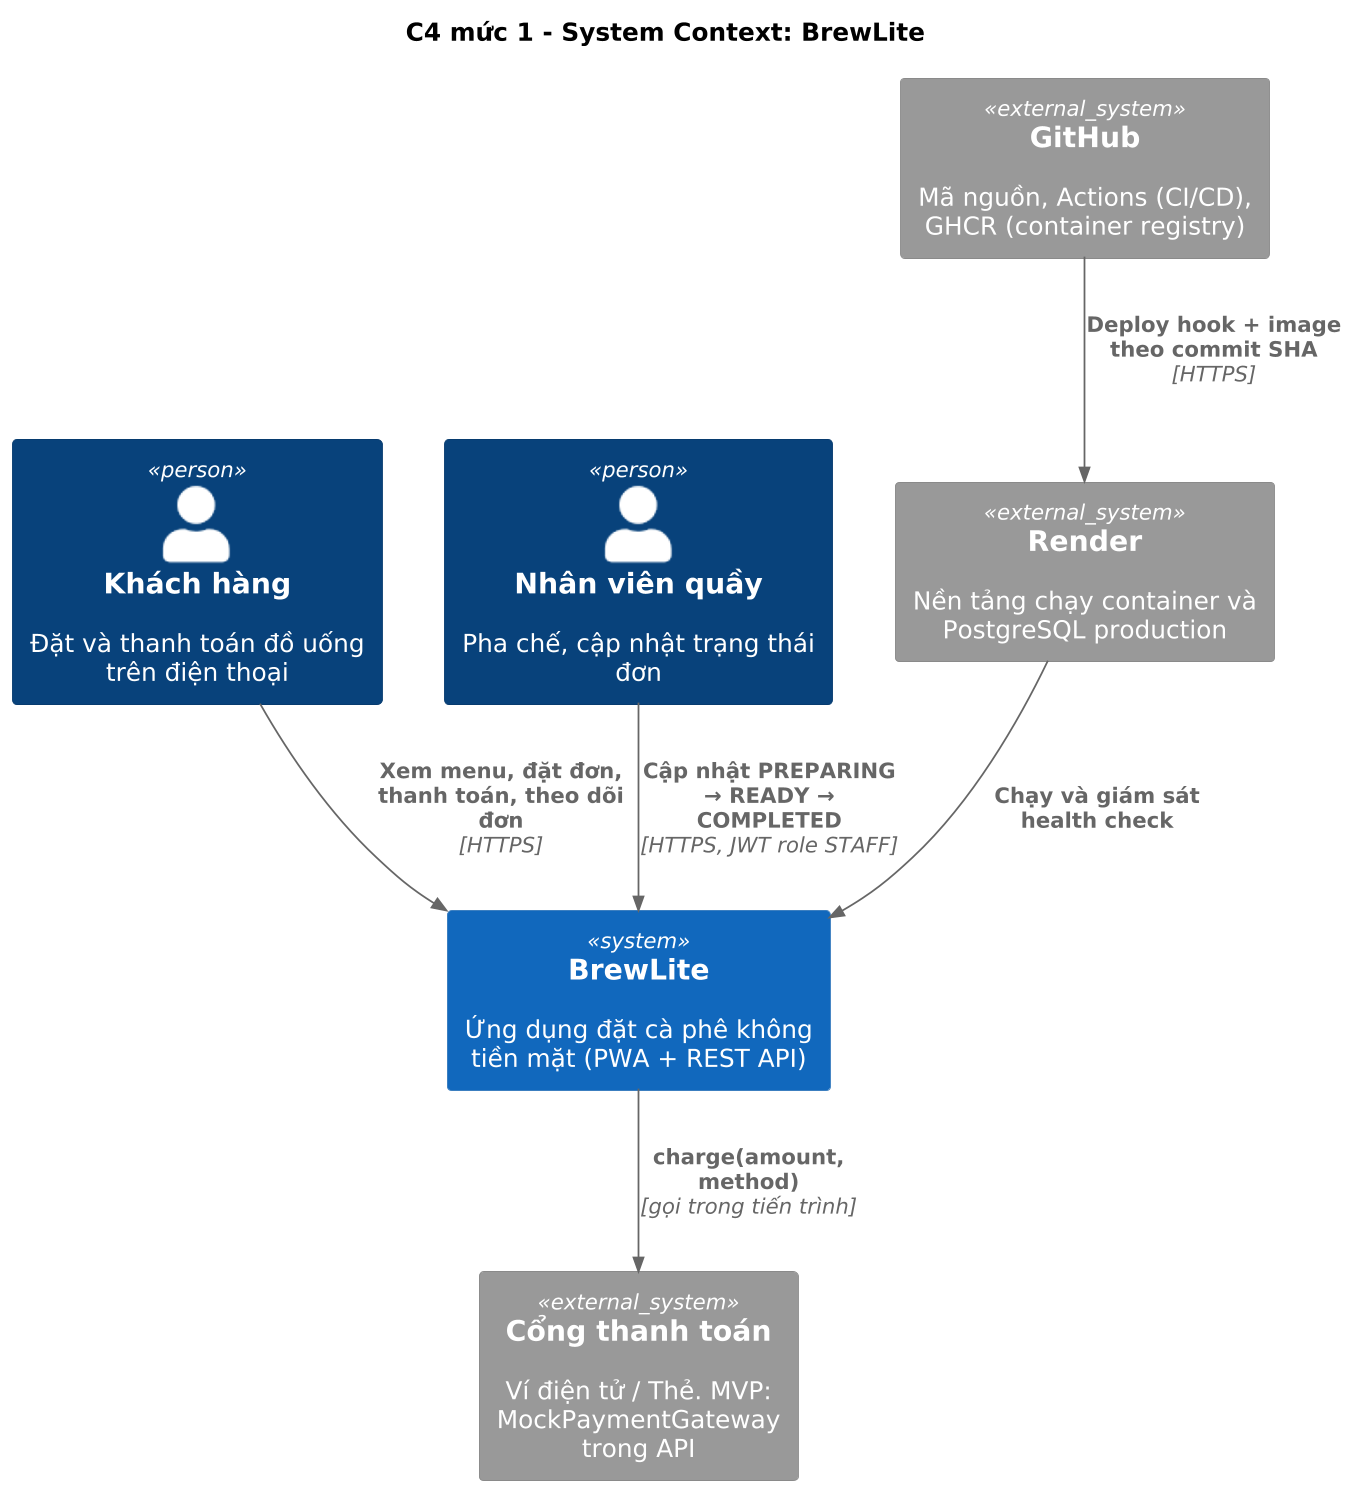
\includegraphics[width=\textwidth,height=0.42\textheight,keepaspectratio]{diagrams/c4-context.png}
\caption{C4 mức 1 -- System Context}
\end{minipage}\hfill
\begin{minipage}[t]{0.46\textwidth}\centering
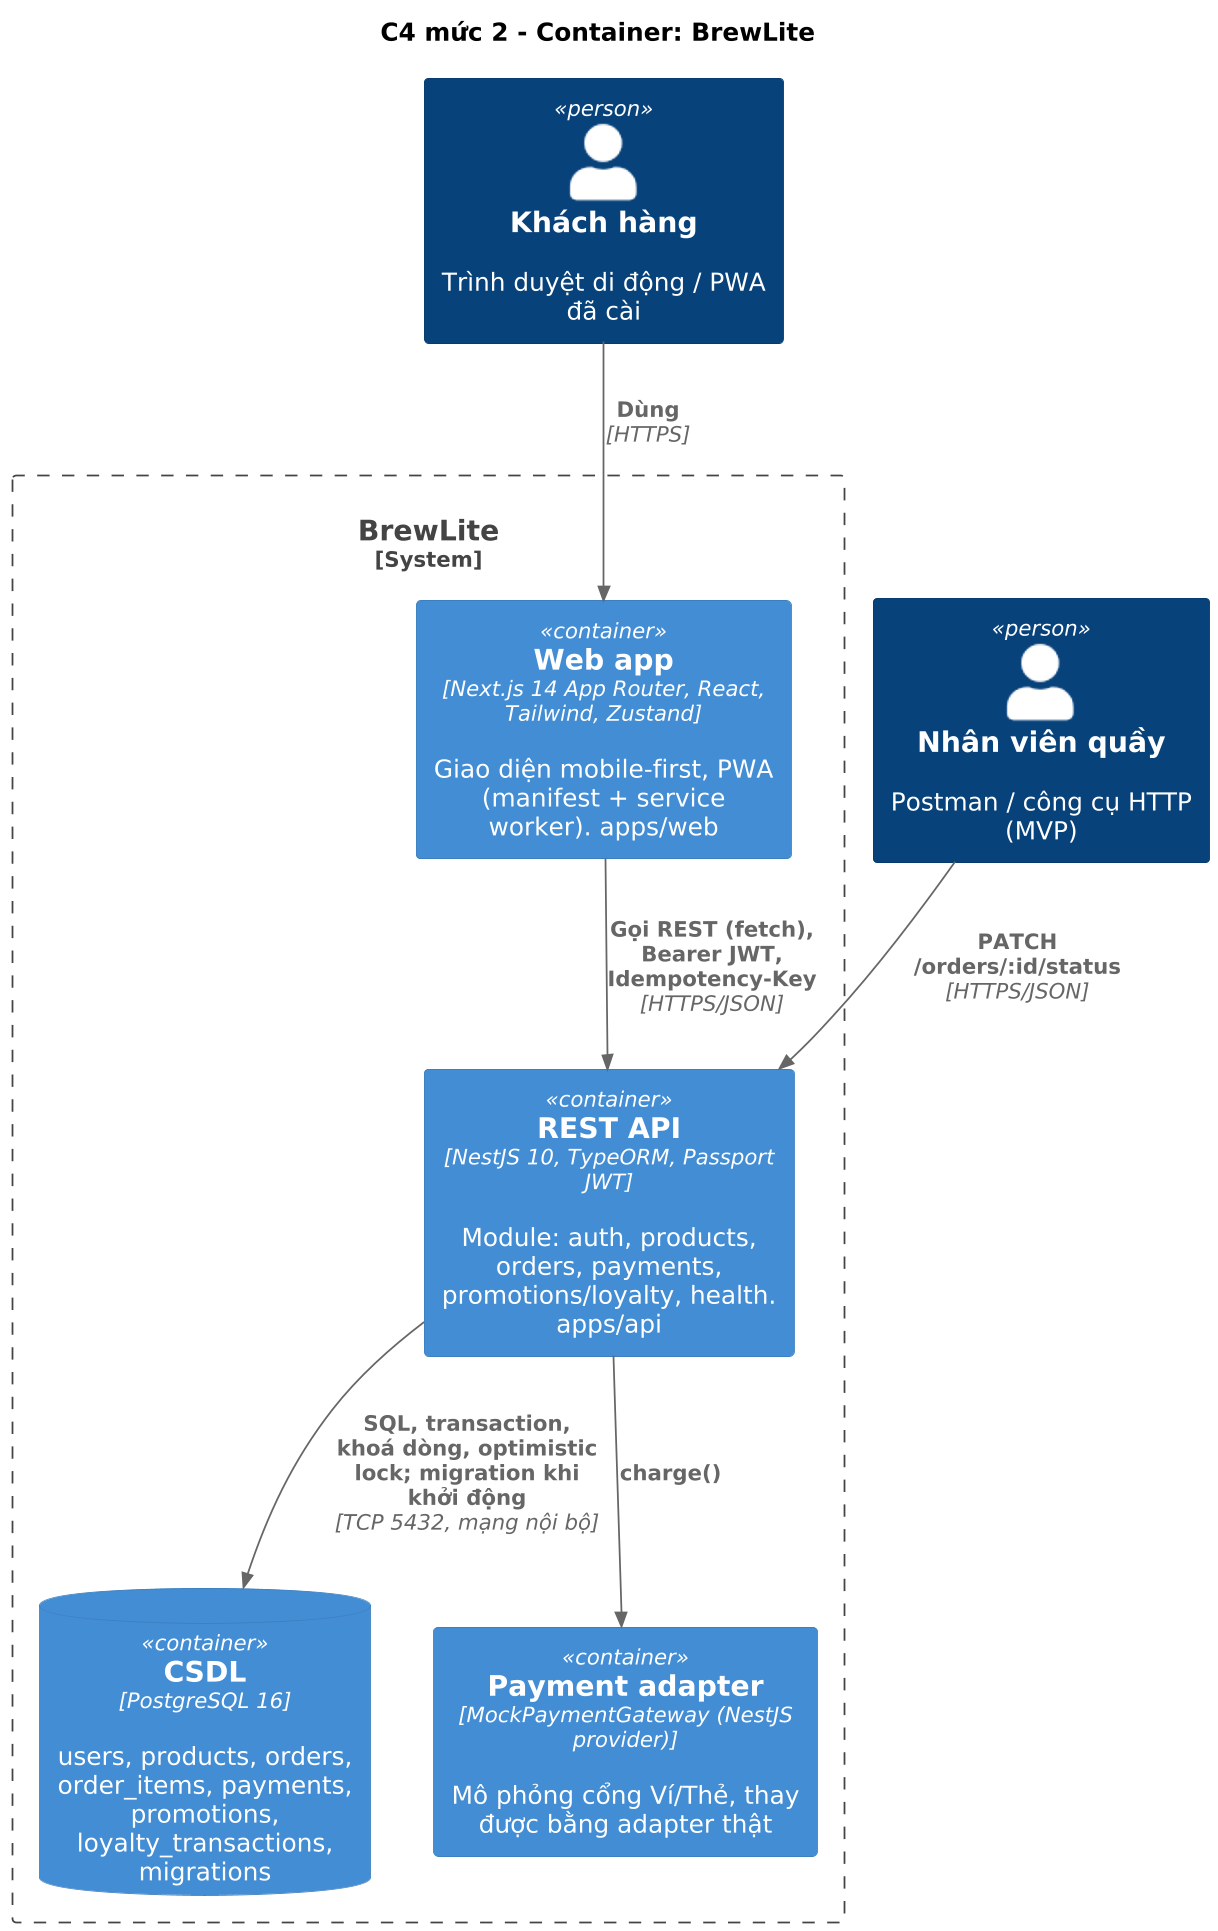
\includegraphics[width=\textwidth,height=0.42\textheight,keepaspectratio]{diagrams/c4-container.png}
\caption{C4 mức 2 -- Container}
\end{minipage}
\end{figure}

\begin{longtable}{|L{2.2cm}|L{3.9cm}|L{3.5cm}|L{5cm}|}
\hline
\textbf{Container} & \textbf{Công nghệ} & \textbf{Production} & \textbf{Trách nhiệm} \\ \hline
\endhead
Web app & Next.js 14 App Router, React 18, Tailwind, Zustand (\st{apps/web}) & Render Web Service \st{brewlite-web} & Giao diện mobile-first, PWA, giỏ hàng phía client, gọi REST API \\ \hline
REST API & NestJS 10, TypeORM, Passport JWT, class-validator (\st{apps/api}) & Render Web Service \st{brewlite-api} & Nghiệp vụ, xác thực, phân quyền, transaction, migration, health check \\ \hline
CSDL & PostgreSQL 16 & Render PostgreSQL \st{brewlite-db} (Internal URL) & Lưu dữ liệu, ràng buộc UNIQUE, CHECK, FK \\ \hline
Payment adapter & \st{MockPaymentGateway} & Trong tiến trình API & Mô phỏng cổng Ví/Thẻ qua interface \st{charge()} \\ \hline
\caption{Các container}
\end{longtable}

\textbf{Frontend Next.js/PWA.} Mỗi màn hình là một route (\st{/}, \st{/products/[id]}, \st{/cart}, \st{/login}, \st{/register}, \st{/checkout}, \st{/orders}, \st{/orders/[id]}) cùng \st{/health} và \st{/manifest.webmanifest}. Mọi màn hình có trạng thái loading, rỗng, lỗi. Zustand + \st{persist} lưu giỏ hàng và phiên. PWA gồm \st{app/manifest.ts}, icon 192/512/maskable, service worker \st{public/sw.js} (network-first cho trang, cache-first cho tài nguyên tĩnh, không cache API) và \st{offline.html}. Next.js chạy chế độ \st{standalone} trong container; tài nguyên \st{/\_next/static} có tên băm nội dung, được trình duyệt và service worker giữ lại; Render Edge kết thúc TLS.

\textbf{Backend NestJS theo module/domain.} Các module \st{auth}, \st{users}, \st{products}, \st{orders}, \st{payments}, \st{promotions}, \st{loyalty}, \st{seed}, \st{health}; thư mục \st{common/} (cấu hình, logger, bảng giá) và \st{database/} (data source, migration). Bên trong theo ba lớp:
\begin{itemize}
  \item \textbf{Presentation:} controller, DTO + class-validator, guard -- không chứa nghiệp vụ.
  \item \textbf{Application/Domain:} service (\st{OrdersService}, \st{PaymentsService}, \st{StockService}, \st{PromotionsService}) và hàm thuần (\st{unitPrice}, \st{computeDiscount}, \st{assertTransition}) được unit test.
  \item \textbf{Infrastructure:} entity TypeORM, migration, \st{MockPaymentGateway}, PostgreSQL.
\end{itemize}

\textbf{PostgreSQL và migration.} Schema chỉ đổi qua migration TypeORM (\st{InitialSchema}, \st{AddRelationsAndChecks}); không dùng \st{synchronize}. API chạy migration khi khởi động với \st{migrationsTransactionMode: 'all'}: mọi migration chưa chạy nằm trong một transaction, lỗi thì rollback, ứng dụng dừng, health check không đạt và Render giữ bản cũ. Integration test xóa schema rồi chạy lại toàn bộ migration ở mỗi lần chạy.

\textbf{Dịch vụ thanh toán mô phỏng.} \st{MockPaymentGateway.charge(\{amount, method, simulateFailure\})} trả \st{\{ok, reference, reason\}}. Nghiệp vụ chỉ phụ thuộc interface này nên thay bằng Momo/VNPay chỉ cần một provider mới.

\textbf{Logging, health check, cấu hình.}
\begin{itemize}
  \item Logging: middleware ghi một dòng mỗi request \st{\{method, path, status, ms\}}, JSON ở production, 5xx mức error, 4xx mức warn, không ghi header/body/query.
  \item Health check: API \st{GET /health} chạy \st{SELECT 1}, đếm migration, trả \st{\{status, db, migrations, version, uptime\}}, 503 khi CSDL lỗi (Hình~\ref{fig:health}); web \st{GET /health} trả \st{\{status, version\}}.
  \item Cấu hình: 12-factor, mọi giá trị qua biến môi trường (\st{.env.example}); production kiểm tra lúc khởi động (\st{DATABASE\_URL}, \st{JWT\_SECRET} $\ge$ 32 ký tự, \st{CORS\_ORIGIN}), thiếu thì dừng.
\end{itemize}

\begin{figure}[H]
\centering
\shot{api-health.png}{0.62\textwidth}
\caption{\st{GET /health} của API (chạy với \st{NODE\_ENV=production})}
\label{fig:health}
\end{figure}

\textbf{Quyết định kiến trúc (ADR).} Mỗi quyết định quan trọng ghi thành một ADR ngắn trong \st{docs/architecture/adr/} (bối cảnh, phương án, quyết định, hệ quả).

\begin{longtable}{|L{3.1cm}|L{3.5cm}|L{3.7cm}|L{4.3cm}|}
\hline
\textbf{ADR} & \textbf{Lý do} & \textbf{Ưu điểm} & \textbf{Hạn chế / trade-off} \\ \hline
\endhead
001 Monorepo \st{apps/web}, \st{apps/api}, \st{docs} & Một người, một pipeline, truy vết trong một repo & Một PR sửa được API, UI, tài liệu, test & Pipeline chạy cả hai app mỗi PR \\ \hline
002 Modular monolith NestJS & Đặt đơn và thanh toán cần transaction ACID chung & Đơn giản, một CSDL, dễ test, rẻ & Không scale độc lập từng domain \\ \hline
003 PostgreSQL + TypeORM + migration & Bắt buộc; cần khóa dòng, UNIQUE, CHECK & Toàn vẹn ở mức CSDL; tái tạo schema được & Phải viết migration mỗi lần đổi entity \\ \hline
004 Migration khi khởi động, một transaction & Gói miễn phí không có pre-deploy; CSDL không public & Không cần bước tay; lỗi thì không chuyển traffic & Migration phải tương thích ngược (expand/contract) \\ \hline
005 Idempotency-Key, khóa dòng, optimistic lock & Rủi ro R-01, R-02 & Không trừ tiền hai lần, không bán vượt kho & Client phải sinh và giữ key \\ \hline
006 Render + GHCR + GitHub Actions & Miễn phí, HTTPS tự động, chạy Docker image, deploy hook nhận image theo SHA & Image bất biến, rollback = deploy lại SHA cũ & Ngủ sau 15 phút; Postgres miễn phí 30 ngày \\ \hline
007 JWT Bearer, bcrypt & Web và API khác origin & Không cần cookie cross-site, CSRF & Token ở localStorage dễ lộ nếu XSS \\ \hline
\caption{Tóm tắt 7 ADR}
\end{longtable}

\subsection{Task 3.2 -- Deployment diagram}
Deploy-01 (Hình~\ref{fig:deploy}) mô tả môi trường production thực tế trên \textbf{Render (region Singapore)} và ranh giới giữa \textbf{LOCAL}, \textbf{CI} và \textbf{PRODUCTION}:
\begin{itemize}
  \item Thiết bị người dùng chạy trình duyệt/PWA, kết nối HTTPS 443 tới Render Edge (TLS tự động).
  \item \st{brewlite-web}: Render Web Service chạy image Next.js (cổng 3000), phục vụ trang và tài nguyên tĩnh.
  \item \st{brewlite-api}: Render Web Service chạy image NestJS (cổng 3001), biến môi trường/secret trong Render Environment, health check \st{/health}, log JSON về Render Logs.
  \item \st{brewlite-db}: Render PostgreSQL 16 có persistent disk, \st{ipAllowList = []} (không public), API kết nối qua Internal URL cổng 5432.
  \item GitHub Actions runner build và đẩy image lên GHCR (container registry), gọi deploy hook bằng secret, chạy smoke test.
\end{itemize}

\dfig[1]{deployment-production.png}{Deploy-01 -- deployment production}{fig:deploy}

\begin{table}[H]
\centering\small
\begin{tabular}{|L{3.5cm}|L{3.6cm}|L{7.6cm}|}
\hline
\textbf{Phần tử Deploy-01} & \textbf{Container} & \textbf{Mã nguồn / cấu hình} \\ \hline
\st{brewlite-web} & Web app & \st{apps/web}, \st{apps/web/Dockerfile}, \st{render.yaml} \\ \hline
\st{brewlite-api} & REST API, Payment adapter & \st{apps/api}, \st{apps/api/Dockerfile}, \st{render.yaml} \\ \hline
\st{brewlite-db} & CSDL & \st{apps/api/src/database}, \st{render.yaml} (\st{databases}) \\ \hline
GHCR & -- & \st{.github/workflows/cd.yml} job \st{image} \\ \hline
GitHub Actions runner & -- & \st{.github/workflows/ci.yml}, \st{cd.yml} \\ \hline
Secret / env & Cấu hình & \st{.env.example}, \st{render.yaml envVars}, GitHub Secrets \\ \hline
Health check, log & Logging, health & \st{health.controller.ts}, \st{app/health/route.ts}, \st{request-logger.ts}, \st{scripts/smoke-test.mjs} \\ \hline
Local & Cả ba & \st{docker-compose.yml} \\ \hline
\end{tabular}
\caption{Truy vết từ deployment diagram tới kiến trúc và mã nguồn}
\end{table}
%%%%%%%%%%%%%%%%%%%% 5. TASK 4 %%%%%%%%%%%%%%%%%%%%
\section{Task 4 -- Triển khai Sprint 1}
\textbf{Sprint Goal:} tạo nền tảng kỹ thuật, tài liệu có kiểm soát phiên bản và một MVP đầu tiên chạy được cho luồng xem menu. Thời gian: 1 tuần, từ 28/10/2026 đến 03/11/2026. Cam kết 11 hạng mục, 27 story point, hoàn thành 27/27.

\subsection{Task 4.1 -- Thiết lập repository}
\begin{Verbatim}[fontsize=\footnotesize,frame=lines,framesep=2mm]
brewlite/
|-- apps/web/        # Next.js mobile-first/PWA (app/, components/, lib/, __tests__/, Dockerfile)
|-- apps/api/        # NestJS (src/, src/database/migrations/, test/unit, test/e2e, Dockerfile)
|-- docs/            # requirements/, diagrams/, architecture/, process/, releases/,
|                    # traceability-matrix.md, deployment.md
|-- tests/e2e/       # Playwright
|-- scripts/         # smoke-test.mjs, create-github-backlog.sh
|-- .github/         # workflows/ci.yml, cd.yml, mẫu PR, mẫu issue, dependabot
|-- docker-compose.yml, render.yaml, .env.example, .gitignore
|-- README.md, CONTRIBUTING.md, CHANGELOG.md
\end{Verbatim}

\begin{itemize}
  \item \textbf{Chiến lược nhánh (GitHub Flow):} \st{main} luôn triển khai được và được bảo vệ (bắt buộc PR, bắt buộc CI xanh, không push thẳng). Nhánh làm việc \st{feat/<issue>-<mô-tả>}, \st{fix/...}, \st{docs/...}, \st{ci/...}. Merge bằng \textit{Squash and merge}; phát hành bằng tag \st{vMAJOR.MINOR.PATCH}.
  \item \textbf{Pull request:} mẫu \st{.github/pull\_request\_template.md} yêu cầu liên kết issue, mã yêu cầu, loại thay đổi, lý do thay đổi tài liệu và checklist Definition of Done.
  \item \textbf{Quy ước commit:} Conventional Commits \st{<type>(<scope>): <mô tả>} với \st{type} $\in$ \{\st{feat, fix, docs, test, refactor, ci, build, chore}\}, ví dụ \st{docs(task2): thêm sequence diagram UC-05}.
  \item \textbf{README.md, .gitignore, .env.example:} README hướng dẫn chạy local, test, build, deploy, rollback; \st{.env} bị bỏ qua; \st{.env.example} liệt kê đủ biến với giá trị local giả.
  \item \textbf{Issue board / Product Backlog:} mẫu issue \textit{User story} và \textit{Lỗi}; backlog Sprint 1 và Sprint 2 trong \st{docs/process/product-backlog.md}; script \st{scripts/create-github-backlog.sh} tạo label, milestone Sprint 1/2 và các issue trên GitHub bằng \st{gh}.
\end{itemize}

\textbf{Definition of Done.} (1) Merge vào \st{main} qua PR dùng mẫu; (2) CI xanh: lint, unit test, build, integration, e2e, quét secret; (3) có test tự động cho hành vi mới, mã test ghi trong ma trận truy vết; (4) backend validate và trả đúng mã lỗi, frontend có loading/rỗng/lỗi; (5) thay đổi schema có migration kèm \st{down()}, tương thích ngược; (6) tài liệu liên quan cập nhật trong cùng PR; (7) không có secret trong mã, log, ảnh; (8) CD triển khai thành công và smoke test đạt.

\begin{longtable}{|c|L{8.2cm}|c|c|L{2.6cm}|}
\hline
\textbf{ID} & \textbf{Hạng mục Sprint 1} & \textbf{Task} & \textbf{SP} & \textbf{Trạng thái} \\ \hline
\endhead
S1-01 & Bối cảnh, stakeholder, phạm vi, giả định, rủi ro & 1.1 & 2 & Done \\ \hline
S1-02 & SRS: FR, NFR, MoSCoW, tiêu chí chấp nhận, use-case tổng quát & 1.2 & 3 & Done \\ \hline
S1-03 & Đặc tả UC-05 & 1.3 & 2 & Done \\ \hline
S1-04 & Activity, sequence, class diagram & 2 & 3 & Done \\ \hline
S1-05 & Kiến trúc C4 + phân lớp, 7 ADR & 3.1 & 3 & Done \\ \hline
S1-06 & Deployment diagram production & 3.2 & 2 & Done \\ \hline
S1-07 & Repo, quy ước, README, \st{.env.example}, DoD & 4.1--4.2 & 2 & Done \\ \hline
S1-08 & API \st{GET /products}, \st{GET /products/:id}, seed & 4.3 & 2 & Done \\ \hline
S1-09 & Màn hình Menu mobile-first với loading/empty/error & 4.3 & 3 & Done \\ \hline
S1-10 & Test API và component Menu & 4.3 & 2 & Done \\ \hline
S1-11 & CI install \ra{} lint \ra{} unit test \ra{} build; bảo vệ nhánh & 4.4 & 3 & Done \\ \hline
& \textbf{Tổng} & & \textbf{27} & \\ \hline
\caption{Sprint Backlog Sprint 1}
\end{longtable}

\subsection{Task 4.2 -- Quản lý tài liệu}
Toàn bộ tạo phẩm Task 1--3 nằm trong \st{docs/} và đi vào repo qua các commit \st{docs(task1)}, \st{docs(task2)}, \st{docs(task3)} trước commit Sprint 1 (Bảng~\ref{tab:history}). Từ đây mọi thay đổi yêu cầu, sơ đồ hoặc kiến trúc phải đi qua pull request; mẫu PR có mục bắt buộc ``Lý do thay đổi tài liệu''. Sơ đồ sửa ở tệp \st{.puml}, kết xuất lại \st{.svg} và commit cả hai trong cùng PR.

\subsection{Task 4.3 -- MVP Sprint 1}
\begin{itemize}
  \item API \st{GET /products} và \st{GET /products/:id} (kèm tùy chọn size/topping), dữ liệu mẫu 8 đồ uống do \st{SeedService} nạp khi bảng rỗng.
  \item Màn hình menu mobile-first bằng Next.js với ba trạng thái loading, empty, error (Hình~\ref{fig:menu-states}).
  \item Kiểm thử: INT-T01 (API sản phẩm), FE-T01 (4 test cho màn hình Menu: loading, danh sách, empty, error + thử lại), FE-T02 (3 test giỏ hàng).
\end{itemize}

\begin{figure}[H]
\centering
\begin{subfigure}[t]{0.235\textwidth}\centering\shot{menu-loading.png}{\textwidth}\caption{Loading}\end{subfigure}\hfill
\begin{subfigure}[t]{0.235\textwidth}\centering\shot{menu-error.png}{\textwidth}\caption{Error + Thử lại}\end{subfigure}\hfill
\begin{subfigure}[t]{0.235\textwidth}\centering\shot{menu-empty.png}{\textwidth}\caption{Empty}\end{subfigure}\hfill
\begin{subfigure}[t]{0.235\textwidth}\centering\shot{menu.png}{\textwidth}\caption{Có dữ liệu}\end{subfigure}
\caption{Màn hình Menu trên khung Pixel 7}
\label{fig:menu-states}
\end{figure}

\subsection{Task 4.4 -- Continuous Integration}
Workflow \st{.github/workflows/ci.yml} chạy tự động khi mở hoặc cập nhật pull request vào \st{main}. Job \st{quality} chạy matrix \st{[api, web]} đúng thứ tự đề yêu cầu \textbf{Install \ra{} Lint \ra{} Unit Test \ra{} Build}; sau đó là integration test với PostgreSQL service container, E2E Playwright và quét secret bằng gitleaks.

\begin{Verbatim}[fontsize=\footnotesize,frame=lines,framesep=2mm]
on:
  pull_request:
    branches: [main]
  workflow_call:          # CD gọi lại làm quality gate
jobs:
  quality:
    strategy: { matrix: { app: [api, web] } }
    defaults: { run: { working-directory: apps/${{ matrix.app }} } }
    steps:
      - uses: actions/checkout@v4
      - uses: actions/setup-node@v4   # Node 22, cache npm
      - name: Install
        run: npm ci
      - name: Lint
        run: npm run lint
      - name: Unit test
        run: npm test
      - name: Build
        run: npm run build
  integration:   # needs: quality; service postgres:16-alpine; npm run test:e2e
  e2e:           # needs: quality; build, chạy API + web, npx playwright test
  secrets:       # gitleaks quét toàn bộ lịch sử git
\end{Verbatim}

\textbf{Chặn merge khi CI lỗi.} Nhánh \st{main} bật branch protection: \textit{Require a pull request before merging} và \textit{Require status checks to pass} với năm check \st{api · install, lint, unit test, build}, \st{web · ...}, \st{api · integration test}, \st{e2e}, \st{quét secret}. Khi một check đỏ, nút Merge bị khóa.

\textbf{Lint phát hiện lỗi thật.} Lần chạy lint đầu tiên trên mã Assignment 1 phát hiện hai import không dùng (\st{ConflictException} trong \st{orders.service.ts}, \st{Order} trong \st{payments.service.ts}); đã sửa trong commit Sprint 1. Thử thêm \st{const unused = 1;} vào \st{main.ts}: lint báo \st{'unused' is assigned a value but never used} và thoát mã lỗi.

\evidenceimg{ci-success.png}{Pull request nhánh \st{docs/sprint-review}: mọi check CI xanh.}
Link: \url{https://github.com/kaiqwwp/brewlite/pulls?q=is:pr+head:docs/sprint-review}

\evidenceimg{ci-fail.png}{Pull request nhánh \st{demo/ci-fail}: bước Lint đỏ, nút Merge bị chặn.}
Link: \url{https://github.com/kaiqwwp/brewlite/pulls?q=is:pr+head:demo/ci-fail}


\textbf{Sprint 1 Review.} Demo tài liệu Task 1--3 trong \st{docs/}, MVP menu chạy bằng \st{docker compose up --build}, tắt API thấy thông báo lỗi và nút Thử lại; PR chạy CI. \textbf{Retrospective:} làm tốt -- tiêu chí chấp nhận gắn mã test ngay từ SRS, lint bắt lỗi sớm, sơ đồ dạng văn bản review được trong PR; cần cải thiện -- Assignment 1 dùng \st{synchronize}, chưa có test frontend, chưa có production; hành động -- chuyển sang migration, giữ Vitest cho component mới, chọn Render + GHCR.

%%%%%%%%%%%%%%%%%%%% 6. TASK 5 %%%%%%%%%%%%%%%%%%%%
\section{Task 5 -- Triển khai Sprint 2, CI/CD và Delivery}
\textbf{Sprint Goal:} hoàn thành luồng end-to-end, tự động hóa đóng gói và triển khai một phiên bản production truy cập được. Thời gian: 1 tuần, từ 04/11/2026 đến 10/11/2026. Cam kết 13 hạng mục, 32 story point.

\subsection{Task 5.1 -- Hoàn thiện MVP}
Chi tiết sản phẩm với size và topping, giỏ hàng và tổng tiền, đăng ký/đăng nhập JWT, tạo đơn, thanh toán Ví/Thẻ mô phỏng, xác nhận, trạng thái và lịch sử đơn được kế thừa từ Assignment 1 và kiểm tra lại bằng E2E. Validate ở cả hai phía: frontend chặn giỏ rỗng, số lượng ngoài 1--20, form đăng ký sai; backend dùng \st{ValidationPipe} (whitelist, \st{forbidNonWhitelisted}) và trả 400/401/403/404/409/402 có thông báo tiếng Việt. Header được sửa để không xuống dòng ở màn hình hẹp khi đã đăng nhập.

\begin{figure}[H]
\centering
\begin{subfigure}[t]{0.19\textwidth}\centering\shot{detail.png}{\textwidth}\caption{Chi tiết, size L}\end{subfigure}\hfill
\begin{subfigure}[t]{0.19\textwidth}\centering\shot{cart.png}{\textwidth}\caption{Giỏ hàng}\end{subfigure}\hfill
\begin{subfigure}[t]{0.19\textwidth}\centering\shot{checkout.png}{\textwidth}\caption{Thanh toán, mã BREW10}\end{subfigure}\hfill
\begin{subfigure}[t]{0.19\textwidth}\centering\shot{confirm.png}{\textwidth}\caption{Xác nhận PAID}\end{subfigure}\hfill
\begin{subfigure}[t]{0.19\textwidth}\centering\shot{orders.png}{\textwidth}\caption{Lịch sử đơn}\end{subfigure}
\caption{Luồng end-to-end trên khung Pixel 7 (chạy bản build production)}
\end{figure}

\subsection{Task 5.2 -- Tích hợp và kiểm thử}
\begin{table}[H]
\centering\small
\begin{tabular}{|L{3.4cm}|L{4.6cm}|c|L{4.2cm}|}
\hline
\textbf{Loại} & \textbf{Phạm vi} & \textbf{Số test} & \textbf{Vị trí / lệnh} \\ \hline
Unit test API & State machine (49 cặp), tính giá, khuyến mãi, điểm, kiểm tra cấu hình & 15 & \st{apps/api/test/unit}, \st{npm test} \\ \hline
Integration test API & HTTP + PostgreSQL thật: auth, tạo đơn, thanh toán, idempotency, tồn kho đồng thời, khuyến mãi, hủy đơn, health, migration, loyalty & 27 & \st{apps/api/test/e2e}, \st{npm run test:integration} \\ \hline
Test component web & Màn hình Menu (4), giỏ hàng (3) & 7 & \st{apps/web}, Vitest \\ \hline
End-to-end & Menu \ra{} chi tiết \ra{} giỏ \ra{} đăng ký \ra{} thanh toán \ra{} xác nhận \ra{} lịch sử, khung Pixel 7 & 1 & \st{tests/e2e}, Playwright \\ \hline
Kiểm thử giao diện (A1) & 55 kịch bản, 224 điểm kiểm tra & 55 & Báo cáo kiểm thử (PDF) trong \st{docs/} \\ \hline
\end{tabular}
\caption{Kiểm thử tự động -- tất cả đạt}
\end{table}

\begin{Verbatim}[fontsize=\footnotesize,frame=lines,framesep=2mm]
$ npm test                      # apps/api
Tests:       15 passed, 15 total
$ npm test                      # apps/web (Vitest)
      Tests  7 passed (7)
$ npm run test:integration      # apps/api, PostgreSQL brewlite_test
Tests:       27 passed, 27 total
$ npm run test:e2e              # Playwright, project mobile-chrome
  ok 1 [mobile-chrome] > E2E-T01 khách đặt và thanh toán một ly từ menu đến xác nhận đơn (1.6s)
  1 passed (2.2s)
\end{Verbatim}

\textbf{Migration và seed tái tạo được CSDL.} Hai migration \st{1794971696733-InitialSchema} và \st{1794971723916-AddRelationsAndChecks} đã được kiểm tra chạy, hoàn tác hai lần rồi chạy lại trên CSDL rỗng; sau đó \st{migration:generate} báo ``No changes in database schema'', chứng tỏ entity và migration khớp nhau. INT-T25 kiểm tra ràng buộc \st{CHK\_products\_stock\_non\_negative} và khóa ngoại bằng cách cố ghi dữ liệu sai.

\textbf{Mô hình dữ liệu mới.} Bảng \st{coupons} đổi thành \st{promotions} (lớp \st{Promotion}); bảng \st{loyalty\_transactions} (lớp \st{LoyaltyTransaction}, \st{UNIQUE(orderId, type)}) ghi mỗi lần cộng/thu hồi điểm; API mới \st{GET /loyalty/me} trả số dư và lịch sử (INT-T26, INT-T27).

\textbf{docker-compose.yml} chạy ba dịch vụ \st{db} (postgres:16-alpine, healthcheck \st{pg\_isready}, volume), \st{api} (chờ db khỏe, cổng 3001) và \st{web} (chờ api khỏe, cổng 3000). Dockerfile chạy bằng user \st{node} và có \st{HEALTHCHECK} gọi \st{/health}.

\textbf{PWA.} Manifest, icon và service worker hoạt động trên bản build production: kiểm tra bằng Playwright thấy service worker \st{/sw.js} đã kích hoạt, icon 512px trả 200, và khi mất mạng trình duyệt nhận trang đã lưu thay vì lỗi kết nối.

\begin{figure}[H]
\centering
\begin{minipage}[t]{0.6\textwidth}\centering\shot{manifest.png}{\textwidth}\par\small (a) \st{/manifest.webmanifest}\end{minipage}\hfill
\begin{minipage}[t]{0.22\textwidth}\centering\shot{offline.png}{\textwidth}\par\small (b) Mất mạng: service worker trả trang đã lưu\end{minipage}
\caption{PWA}
\end{figure}

\subsection{Task 5.3 -- Continuous Delivery/Deployment}
Workflow \st{.github/workflows/cd.yml} chạy khi push vào \st{main}, khi đẩy tag \st{vX.Y.Z}, hoặc chạy tay với tham số \st{rollback\_to}.

\begin{center}
\begin{tikzpicture}[node distance=0.25cm, every node/.style={draw=brew, rounded corners, fill=brew!8, font=\scriptsize, align=center, minimum height=0.9cm, text width=1.55cm}]
\node (a) {Push / Tag};
\node[right=of a] (b) {Lint và Test\\(gọi ci.yml)};
\node[right=of b] (c) {Build};
\node[right=of c] (d) {Docker Image\\tag = SHA};
\node[right=of d] (e) {Push GHCR};
\node[right=of e] (f) {Deploy\\(Render hook)};
\node[right=of f] (g) {Smoke Test};
\foreach \x/\y in {a/b,b/c,c/d,d/e,e/f,f/g} \draw[-{Stealth}, brew] (\x) -- (\y);
\node[below=0.5cm of f, fill=warnred!8, draw=warnred] (r) {Rollback\\về SHA trước};
\draw[-{Stealth}, warnred, dashed] (g) |- (r);
\end{tikzpicture}
\end{center}

\begin{longtable}{|L{4.6cm}|L{10.4cm}|}
\hline
\textbf{Yêu cầu của đề} & \textbf{Cách thực hiện} \\ \hline
\endhead
1. Quality gate lint, test, build & Job \st{quality-gate} gọi lại \st{ci.yml} (\st{workflow\_call}); job sau chỉ chạy khi gate xanh \\ \hline
2. Image tag commit SHA hoặc semver & \st{docker/metadata-action}: \st{type=sha,format=long} (\st{ghcr.io/kaiqwwp/brewlite-api:<sha>}), \st{type=semver} khi đẩy tag, \st{latest} cho \st{main} \\ \hline
3. Push lên container registry & \st{docker/build-push-action} đẩy lên GHCR, đăng nhập bằng \st{GITHUB\_TOKEN}; image chứa \st{APP\_VERSION=<sha>} \\ \hline
4. Triển khai bằng secret của CI & \st{RENDER\_DEPLOY\_HOOK\_API}, \st{RENDER\_DEPLOY\_HOOK\_WEB} là secret của environment \st{production}; gọi hook kèm \st{imgURL=<image:sha>}; GitHub che giá trị secret trong log \\ \hline
5. Chạy migration an toàn & Migration chạy khi container API mới khởi động, trong một transaction; lỗi thì container dừng, Render không chuyển traffic khỏi bản cũ (ADR-004). Quy tắc migration tương thích ngược để rollback image an toàn \\ \hline
6. Health check / smoke test & \st{scripts/smoke-test.mjs}: chờ API \st{/health} báo đúng SHA vừa deploy và \st{db: up}, rồi deploy web; kiểm tra \st{GET /products}, web \st{/health} đúng SHA, trang Menu, manifest PWA; có thử lại vì dịch vụ cần thời gian khởi động \\ \hline
7. Dừng pipeline và rollback & Trước khi deploy, pipeline đọc \st{version} đang chạy từ \st{/health}. Nếu deploy hoặc smoke test lỗi, bước \textit{Rollback} gọi lại deploy hook với image của SHA đó, chạy smoke test rồi kết thúc với trạng thái lỗi. Rollback tay: chạy CD với \st{rollback\_to=<SHA>}, hoặc nút Rollback trong Render \\ \hline
\caption{Pipeline CD đáp ứng 7 yêu cầu}
\end{longtable}

Smoke test được thử trên máy local với API chạy \st{NODE\_ENV=production}: đúng phiên bản thì đạt cả năm kiểm tra; truyền sai phiên bản mong đợi thì báo ``đang chạy local-test, chờ wrongsha'' và thoát mã 1, đây là tín hiệu kích hoạt rollback.

\evidenceimg{cd-success.png}{Lần chạy CD thành công trên \st{main} sau khi merge PR \#13: sơ đồ job và Summary ``Production đang chạy 261da37...''.}
Link: \url{https://github.com/kaiqwwp/brewlite/actions/workflows/cd.yml?query=branch:main+is:success}

\evidenceimg{rollback.png}{Rollback: chạy CD với \st{rollback\_to} = \st{1aade28}; \st{/health} trả về SHA cũ \st{1aade28}, sau đó triển khai lại bản \st{v2.0.0} (\st{261da37}).}
Link: \url{https://github.com/kaiqwwp/brewlite/actions/workflows/cd.yml?query=event:workflow_dispatch}


\subsection{Task 5.4 -- Triển khai và bàn giao}
\begin{longtable}{|L{5cm}|L{10cm}|}
\hline
\textbf{Yêu cầu bàn giao} & \textbf{Kết quả} \\ \hline
\endhead
URL frontend production qua HTTPS & \url{https://brewlite-web-ed96.onrender.com} \\ \hline
URL API và health check & \url{https://brewlite-api-9uli.onrender.com/health} \\ \hline
CSDL production không public & Render PostgreSQL với \st{ipAllowList: []}; API dùng Internal URL qua \st{fromDatabase} trong \st{render.yaml} \\ \hline
Secret không có trong repo/log & \st{.env} bị bỏ qua; \st{JWT\_SECRET} do Render sinh (\st{generateValue}); deploy hook là secret GitHub; gitleaks quét lịch sử git: không phát hiện secret \\ \hline
Release/tag và release notes & Tag \st{v1.0.0} (Assignment 1); tag \st{v2.0.0} kích hoạt CD và job \st{release} tạo GitHub Release từ \st{docs/releases/v2.0.0.md}; \st{CHANGELOG.md} \\ \hline
README chạy local, test, build, deploy, rollback & \st{README.md} mục 1--4 và \st{docs/deployment.md} (thiết lập GitHub, Render, phát hành, rollback, minh chứng) \\ \hline
Video/demo end-to-end & \url{https://github.com/kaiqwwp/brewlite/blob/main/docs/evidence/video.md} \\ \hline
Sprint Review và Retrospective & Mục \ref{sec:review} và \st{docs/process/sprint-2.md} \\ \hline
\caption{Bàn giao}
\end{longtable}

Kiểm tra ``một người không thuộc nhóm có thể clone và chạy theo README'': repository được clone vào thư mục trống, chạy \st{npm run install:all}, \st{npm run lint}, \st{npm test}, \st{npm run test:integration}, \st{npm run build} theo đúng README -- tất cả thành công.

\subsubsection{Sprint 2 Review và Retrospective}\label{sec:review}
\begin{longtable}{|L{4.4cm}|L{7cm}|L{3.6cm}|}
\hline
\textbf{Hạng mục demo} & \textbf{Kết quả} & \textbf{Minh chứng} \\ \hline
\endhead
Luồng end-to-end trên điện thoại & Menu \ra{} chi tiết \ra{} giỏ \ra{} đăng ký \ra{} thanh toán Ví \ra{} ``Đã thanh toán'' \ra{} lịch sử & E2E-T01, video \\ \hline
Thanh toán lỗi và thử lại & Bật ``Mô phỏng thanh toán lỗi'' \ra{} \st{PAYMENT\_FAILED} \ra{} thử lại \ra{} \st{PAID} & INT-T09, video \\ \hline
Migration, health & \st{/health}: \st{db: up}, \st{migrations: 2}, \st{version: <SHA>} & INT-T24, smoke test \\ \hline
CI/CD, rollback & Merge PR \ra{} image SHA trên GHCR \ra{} Render \ra{} smoke test; rollback bằng \st{rollback\_to} & Link CD \\ \hline
\caption{Sprint 2 Review}
\end{longtable}
Phản hồi của Product Owner (đóng vai quản lý cửa hàng): luồng đặt và thanh toán trên điện thoại đủ nhanh để dùng tại quầy, thông báo khi thanh toán lỗi rõ ràng và thử lại được ngay. Đề nghị cho bản sau: màn hình riêng cho nhân viên quầy đổi trạng thái đơn (hiện phải gọi API) và báo cho khách khi đơn chuyển sang \st{READY}. Hai đề nghị được đưa vào Product Backlog.

\begin{table}[H]
\centering\small
\begin{tabular}{|L{4.7cm}|L{4.7cm}|L{4.9cm}|}
\hline
\textbf{Làm tốt} & \textbf{Cần cải thiện} & \textbf{Hành động tiếp theo} \\ \hline
Pipeline xác nhận đúng commit SHA đang chạy qua \st{/health} trước khi báo thành công & Gói miễn phí Render ngủ sau 15 phút làm smoke test chậm & Giữ cơ chế thử lại; cân nhắc gói trả phí khi demo thật \\ \hline
Ràng buộc CSDL (CHECK, FK, UNIQUE) bắt lỗi ở tầng thấp nhất & Chưa có giao diện nhân viên & Đưa giao diện barista lên Sprint kế tiếp \\ \hline
E2E chạy trên khung điện thoại phát hiện lỗi bố cục header & JWT lưu trong localStorage & Chuyển sang cookie HttpOnly + refresh token \\ \hline
\end{tabular}
\caption{Sprint 2 Retrospective}
\end{table}

%%%%%%%%%%%%%%%%%%%% 7. TRUY VẾT %%%%%%%%%%%%%%%%%%%%
\section{Truy vết}
Bảng đầy đủ (kèm NFR và user story bổ sung US-10..US-14) nằm trong \st{docs/traceability-matrix.md}. Bảng dưới là phần yêu cầu chức năng.

{\small
\begin{longtable}{|L{2.2cm}|L{2.5cm}|L{3cm}|L{3.7cm}|L{2.9cm}|}
\hline
\textbf{Mã yêu cầu} & \textbf{Use-case / User Story} & \textbf{Thiết kế / Sơ đồ} & \textbf{Code / API} & \textbf{Test} \\ \hline
\endhead
FR-01 Xem menu & UC-01, US-01 & Activity-01, Class-01 & \st{GET /products} & INT-T01, FE-T01, E2E-T01 \\ \hline
FR-02 Chi tiết, size, topping & UC-02, US-02 & Activity-01, Class-01 & \st{GET /products/:id}, \st{unitPrice()} & INT-T01, UT-05..07 \\ \hline
FR-03 Giỏ hàng & UC-03, US-03 & Activity-01 & \st{lib/store.ts} & FE-T02, UI-B \\ \hline
FR-04 Xác thực JWT & UC-04, US-04 & Activity-01, Sequence-01, ADR-007 & \st{/auth/register}, \st{/auth/login}, \st{/auth/me} & INT-T02..04, E2E-T01 \\ \hline
FR-05 Đặt đơn & UC-05, US-07, US-08 & Sequence-01, Activity-01, Class-01, ADR-005 & \st{POST /orders}, \st{stock.service.ts} & INT-T05, T06, T14, T15, T18--T20, T25 \\ \hline
FR-06 Mã giảm giá & UC-06, US-09 & Class-01 \st{Promotion} & \st{computeDiscount()} & UT-08..10, INT-T21, T23 \\ \hline
FR-07 Thanh toán & UC-05, UC-07, US-05, US-07 & Sequence-01, Activity-01, ADR-005 & \st{POST /payments} & INT-T08..10, T16, T17 \\ \hline
FR-08 Xác nhận & UC-08, US-06 & Sequence-01 & \st{GET /orders/:id} & E2E-T01, UI-E \\ \hline
FR-09 Lịch sử & UC-08, US-06 & Activity-01 & \st{GET /orders/me} & INT-T07, E2E-T01 \\ \hline
FR-10 Trạng thái đơn & UC-11, US-10 & Class-01 \st{OrderStatus} & \st{PATCH /orders/:id/status}, \st{assertTransition} & UT-01..04, INT-T11, T12 \\ \hline
FR-11 Hủy đơn & UC-09, US-11 & Activity-01 & \st{POST /orders/:id/cancel} & INT-T13, T22 \\ \hline
FR-12 Điểm thưởng & UC-10, US-09, US-13 & Class-01 \st{LoyaltyTransaction}, Sequence-01 & \st{awardPoints}, \st{revokePoints}, \st{GET /loyalty/me} & UT-11, INT-T16, T21, T22, T26, T27 \\ \hline
FR-13 PWA & UC-12, US-12 & C4-02, Deploy-01 & \st{manifest.ts}, \st{sw.js} & Smoke test \\ \hline
\caption{Ma trận truy vết yêu cầu chức năng}
\end{longtable}
}

%%%%%%%%%%%%%%%%%%%% 8. KẾT LUẬN %%%%%%%%%%%%%%%%%%%%
\section{Kết luận}
\subsection{Kết quả}
Assignment 2 đã đưa BrewLite từ một ứng dụng chạy bằng Docker Compose ở máy cá nhân thành một sản phẩm có đủ chuỗi tạo phẩm từ yêu cầu đến triển khai: SRS có tiêu chí chấp nhận kiểm chứng được, ba loại sơ đồ nhất quán với mã nguồn, kiến trúc có quyết định ghi lại, CSDL quản lý bằng migration, 50 test tự động chạy trong CI, pipeline CD build image theo commit SHA, triển khai, smoke test và tự rollback, cùng ma trận truy vết nối mỗi yêu cầu tới thiết kế, mã và test.

\subsection{Hạn chế}
\begin{itemize}
  \item Gói miễn phí Render: dịch vụ ngủ sau 15 phút không dùng, PostgreSQL miễn phí hết hạn sau 30 ngày.
  \item Cổng thanh toán là mô phỏng, chưa có hoàn tiền khi hủy đơn đã thanh toán; đơn \st{PENDING} chưa tự hết hạn.
  \item Chưa có giao diện nhân viên quầy (chỉ có API); JWT lưu trong localStorage.
  \item E2E chỉ chạy trên Chromium; chưa kiểm thử tải.
\end{itemize}

\subsection{Hướng phát triển}
Giao diện barista và thông báo thời gian thực khi đơn \st{READY}; cổng thanh toán thật với webhook và hoàn tiền; đơn \st{PENDING} hết hạn sau 15 phút; cookie HttpOnly và refresh token; rate limit cho \st{/auth}; chạy migration bằng job pre-deploy khi nâng gói; kiểm thử tải với k6.

%%%%%%%%%%%%%%%%%%%% PHỤ LỤC %%%%%%%%%%%%%%%%%%%%
\appendix
\section{Checklist nộp bài}
\begin{longtable}{|L{6.3cm}|c|L{6.6cm}|}
\hline
\textbf{Mục} & \textbf{Trạng thái} & \textbf{Vị trí} \\ \hline
\endhead
Link repository và quyền truy cập cho giảng viên & \checkmark & \url{https://github.com/kaiqwwp/brewlite}; repo public hoặc mời giảng viên quyền Read \\ \hline
SRS, đặc tả use-case, ma trận truy vết & \checkmark & \st{docs/requirements/}, \st{docs/traceability-matrix.md} \\ \hline
Activity, sequence, class, deployment diagram & \checkmark & \st{docs/diagrams/} (\st{.puml} + \st{.svg}) \\ \hline
Source code frontend, backend, migration & \checkmark & \st{apps/web}, \st{apps/api}, \st{apps/api/src/database/migrations} \\ \hline
Unit, integration, end-to-end test & \checkmark & 15 + 27 + 7 + 1 test \\ \hline
Pipeline CI/CD chạy thành công & \checkmark & \st{.github/workflows}; \url{https://github.com/kaiqwwp/brewlite/actions/workflows/cd.yml?query=branch:main+is:success} \\ \hline
URL production, API, health check & \checkmark & Mục 1.2 \\ \hline
Release notes, README, hướng dẫn rollback & \checkmark & \st{docs/releases/}, \st{README.md}, \st{docs/deployment.md} \\ \hline
Video/demo và Sprint Retrospective & \checkmark & \url{https://github.com/kaiqwwp/brewlite/blob/main/docs/evidence/video.md}; \st{docs/process/sprint-2.md} \\ \hline
\caption{Checklist nộp bài (mục 9.1 của đề)}
\end{longtable}

\section{Hướng dẫn chạy nhanh}
\begin{Verbatim}[fontsize=\footnotesize,frame=lines,framesep=2mm]
# Local bằng Docker
git clone https://github.com/kaiqwwp/brewlite.git && cd brewlite
docker compose up --build          # web :3000, API :3001, /health
# Kiểm thử
npm run install:all && npm run lint && npm test
createdb brewlite_test && npm run test:integration
npm run build && npm run test:e2e  # cần hệ thống đang chạy
# Smoke test production
npm run smoke -- https://<api> https://<web>
# Phát hành và rollback
git tag -a v2.0.0 -m "BrewLite 2.0.0" && git push origin v2.0.0
# GitHub > Actions > CD > Run workflow > rollback_to=<SHA>
\end{Verbatim}

\end{document}
